% Artículo del Proyecto Integrador (Producto de difusión) — Equipo 1
% Formato: carta, una columna, 11 pt, márgenes de 2.5 cm, interlineado 1.15.
% Referencias: APA 7. Compila con pdfLaTeX + Biber (latexmk -pdf articulo.tex).
% Archivos necesarios en la misma carpeta: logo.jpeg, fig_*.png y referencias.bib
\documentclass[letterpaper,11pt]{article}

% --- Idioma y tipografía ---
\usepackage[T1]{fontenc}
\usepackage{lmodern}
\usepackage[spanish,es-tabla,es-nodecimaldot]{babel}

% --- Página: carta, márgenes 2.5 cm, interlineado 1.15 ---
\usepackage[margin=2.5cm]{geometry}
\geometry{headheight=52pt,headsep=0.3cm}
\usepackage{setspace}
\setstretch{1.15}

% --- Figuras, tablas y matemáticas ---
\usepackage{graphicx}
\usepackage{booktabs}
\usepackage{float}
\usepackage{array}
\usepackage{amsmath,amssymb}
\emergencystretch=1.5em
\usepackage{xcolor}
\usepackage[font=small,labelfont=bf,labelsep=colon]{caption}
\usepackage{enumitem}
\setlist{itemsep=1pt,topsep=3pt}
\usepackage{tikz}
\usetikzlibrary{positioning,arrows.meta,fit,backgrounds}

% --- Encabezado: logo (logo.jpeg) solo en la primera página ---
\usepackage{fancyhdr}
\renewcommand{\headrulewidth}{0pt}
\fancypagestyle{plain}{%
  \fancyhf{}%
  \fancyhead[C]{
\includegraphics[height=1.2cm]{logo.jpeg}}%
  \fancyfoot[C]{\thepage}}
\pagestyle{fancy}
\fancyhf{}
\fancyfoot[C]{\thepage}

% --- Encabezados de sección ---
\usepackage{titlesec}
\titleformat{\section}{\Large\bfseries}{\thesection.}{0.6em}{}
\titleformat{\subsection}{\large\bfseries}{\thesubsection.}{0.6em}{}
\titlespacing*{\section}{0pt}{1.6ex plus 0.4ex minus 0.2ex}{1ex}

% --- Referencias: APA 7 ---
\usepackage{csquotes}
\usepackage[style=apa,backend=biber]{biblatex}
\addbibresource{referencias.bib}

% --- Enlaces y URL (DOI); se carga al final ---
\usepackage[hidelinks]{hyperref}
\urlstyle{same}

% --- Atajos ---
\newcommand{\act}[1]{\texttt{#1}}
\newcommand{\pend}[1]{\textcolor{red}{[#1]}}

% --- Título ---
\title{\textbf{Preentrenamiento autosupervisado con codificación predictiva contrastiva para reconocer actividades de manejo manual de cargas}}
\author{Isaura Yutsil Flores Escamilla\quad Paola Alejandra León Guarneros\\[2pt] Dylan Ulises Quiroz Hernández\\[6pt]
  \normalsize Proyecto Integrador $\cdot$ Maestría en Inteligencia Artificial Aplicada \\[6pt]
  \normalsize Asesor: Gerardo Jesús Camacho González \quad$\cdot$\quad 10 de octubre de 2026}
\date{\vspace{-2ex}}

\begin{document}

\maketitle

% --- Resumen ---
\begin{abstract}
\noindent
Reconocer automáticamente las actividades de manejo manual de cargas es el primer paso para evaluar su riesgo ergonómico, pero los modelos supervisados exigen anotar cada actividad, y esa anotación es la parte más cara de llevar un sistema a una planta. Este trabajo de investigación evalúa si la codificación predictiva contrastiva (CPC), un preentrenamiento que aprende sin etiquetas, reduce esa dependencia. Se usó un conjunto público de 14 personas que realizan siete actividades con cargas de 2 a 12~kg, registradas con electromiografía de superficie (sEMG) y con un traje inercial de 17 sensores. Todos los modelos se evaluaron dejando fuera a una persona a la vez (LOSO) con los sujetos 1--12. La sEMG del brazo se quedó en un F1 macro de 0.44--0.49, mientras que la captura de movimiento alcanzó 0.88--0.89, por lo que el proyecto se reorientó hacia el movimiento. El modelo final es una red CPC con encoder convolucional causal y GRU, que usa 10 variables de 11 sensores inerciales. Con todas las etiquetas obtiene un F1 macro de $0.873 \pm 0.036$, cerca del Random Forest de referencia ($0.892$). Con 10 ventanas etiquetadas por actividad o menos, lo supera por 0.04 a 0.11 de F1 en 11 o 12 de los 12 sujetos, una ventaja que se debe al preentrenamiento y que equivale a usar alrededor de la mitad de las etiquetas. Se recomienda CPC cuando hay mucho movimiento registrado y pocas anotaciones; la evaluación con los dos sujetos reservados sigue pendiente.
\end{abstract}

\noindent\textbf{Palabras clave:} reconocimiento de actividades humanas, aprendizaje autosupervisado, codificación predictiva contrastiva, sensores inerciales, ergonomía.

% =====================================================================
\section{Contexto y problema de investigación}
% =====================================================================

\subsection{Motivación}
El manejo manual de cargas (levantar, sostener, transportar y colocar objetos) es una de las tareas industriales más asociadas con lesiones musculoesqueléticas. Evaluar su riesgo requiere saber \emph{qué} actividad realiza el trabajador y \emph{cuándo}: no pesa lo mismo levantar una carga desde el piso que tomarla de una mesa. Hoy esa segmentación suele hacerse revisando video, una tarea lenta que no escala a jornadas completas.

El reconocimiento de actividades humanas (HAR, por sus siglas en inglés) con sensores corporales permite automatizarla. Sin embargo, los modelos supervisados dependen de grandes volúmenes de datos anotados. En HAR, grabar horas de movimiento es barato, pero etiquetarlas instante por instante es caro \parencite{haresamudram2021}. Por eso conviene preguntarse si un modelo puede aprender primero de los datos sin etiquetar y necesitar después pocas anotaciones.

La codificación predictiva contrastiva (CPC) \parencite{vandenoord2018} responde a esa necesidad. Una red aprende a representar una señal resolviendo una tarea que no requiere etiquetas: a partir del pasado, reconocer cuál es el futuro real entre varios candidatos. \textcite{haresamudram2021} la aplicaron a HAR con acelerómetros y reportaron que, con todas las etiquetas, CPC queda a la par del entrenamiento supervisado, y que su ventaja aparece cuando las etiquetas escasean.

\subsection{Pregunta de investigación y objetivos}
Este proyecto no resuelve un problema de negocio definido por un cliente: es un trabajo de investigación aplicada. La pregunta que lo guía es:

\begin{quote}
\emph{¿Puede un modelo preentrenado sin etiquetas con CPC reconocer las actividades de manejo manual de cargas de una persona nueva con un desempeño comparable al de un modelo supervisado, y superarlo cuando las etiquetas son escasas?}
\end{quote}

\noindent Los objetivos específicos fueron:
\begin{enumerate}
  \item identificar qué fuente de señal (sEMG, captura de movimiento o ambas) permite distinguir las siete actividades;
  \item comparar CPC con modelos supervisados clásicos y profundos bajo un mismo protocolo que evalúa a personas no vistas;
  \item determinar el mínimo de variables y sensores que conserva el desempeño, como requisito para un sistema portátil;
  \item medir el desempeño de CPC frente al modelo supervisado cuando sólo se dispone de pocas ventanas etiquetadas.
\end{enumerate}

\subsection{Cambio de enfoque}
El planteamiento inicial (Avance~0) proponía aplicar CPC con redes recurrentes xLSTM \parencite{beck2024} a la \emph{electromiografía de superficie} (sEMG) de los brazos. Los Avances~1 a~3 mostraron que la sEMG, por sí sola, se queda en un F1 macro de 0.44--0.49 con cualquier modelo (Sección~\ref{sec:semg}). La sEMG mide \emph{cuánto} esfuerzo hace el músculo, pero no \emph{dónde} está el cuerpo, y levantar desde el piso o desde la mesa activa los mismos músculos. Al incorporar la captura de movimiento de cuerpo completo, el F1 subió a $\approx 0.88$, y la sEMG dejó de aportar información medible (Sección~\ref{sec:fuente}).

El enfoque adoptado finalmente fue: \textbf{CPC con red de contexto GRU sobre variables de movimiento}, reducidas después a las que pueden medir 11 sensores inerciales, con el énfasis en el escenario de \textbf{pocas etiquetas}. La xLSTM se conservó como candidata en la comparación de modelos, pero no fue la mejor opción.

% =====================================================================
\section{Datos y preparación}
% =====================================================================

\subsection{Conjunto de datos}
Se usó el \emph{Manual Material Handling Dataset for Biomechanical and Ergonomics Analysis} \parencite{bassani2021dataset}, publicado en Zenodo con licencia CC~BY~4.0. Incluye a 14 sujetos (12 hombres y 2 mujeres, de 25 a 38 años), cada uno con 37 ensayos isocinéticos, bimanuales y unilaterales, con cargas de 2 a 12~kg. Cada ensayo se registró con dos sistemas:

\begin{itemize}
  \item \textbf{sEMG:} 8 canales en el miembro superior, 643 ensayos (13.2~h), con frecuencias de muestreo de 367 a 1006~Hz según el archivo.
  \item \textbf{Captura de movimiento (MVNX):} traje inercial Xsens MVN de 17 sensores a 240~Hz, con un modelo corporal de 23 segmentos y 22 articulaciones (782 columnas por instante): posición, velocidad, aceleración, orientación, ángulos articulares y contacto de los pies.
\end{itemize}

Las etiquetas distinguen las siete actividades de la Tabla~\ref{tab:clases}. Sólo alrededor del 67\,\% de cada grabación está anotado, y la postura neutral ocupa el 43\,\% del tiempo etiquetado.

\begin{table}[H]
  \centering
  \small
  \caption{Actividades por reconocer y proporción de ventanas etiquetadas (sujetos 1--12, 40\,944 ventanas).}
  \label{tab:clases}
  \begin{tabular}{llr}
    \toprule
    Código & Actividad & \% de ventanas \\
    \midrule
    \act{N}  & Postura neutral              & 43.9 \\
    \act{LF} & Levantar desde el piso       & 8.8 \\
    \act{K}  & Mantener la carga levantada  & 8.4 \\
    \act{PT} & Colocar en la mesa           & 15.3 \\
    \act{LT} & Levantar desde la mesa       & 9.7 \\
    \act{W}  & Caminar con la carga         & 7.2 \\
    \act{PF} & Colocar en el piso           & 6.7 \\
    \bottomrule
  \end{tabular}
\end{table}

\subsection{Exploración y preparación de la sEMG (Avances 1 y 2)}
La exploración no encontró valores nulos, huecos ni canales constantes, pero sí tres ensayos del sujeto~7 con canales dañados, dos archivos con etiquetas inconsistentes y un ensayo faltante del sujeto~12. Como la frecuencia de muestreo varía entre archivos, los registros no pueden combinarse por número de muestras. La preparación fue:

\begin{enumerate}
  \item excluir los ensayos dañados o con etiquetas inconsistentes;
  \item usar la envolvente normalizada \texttt{Norm\_RMS} (\% de la contracción voluntaria máxima) de los 8 canales;
  \item aplicar un filtro antialias y remuestrear a \textbf{12~Hz}, que rindió igual que 25~Hz con un tercio del costo;
  \item recortar por cuantiles, aplicar \texttt{log1p} y escalar con \texttt{RobustScaler}, ajustado sólo con los sujetos de entrenamiento.
\end{enumerate}

Para los modelos clásicos, el Avance~2 construyó un catálogo de \textbf{202 características por ventana} (nivel, dinámica, dispersión, espectro y coactivación de los canales). La exploración confirmó que la sEMG separa claramente el reposo de la actividad y que crece con la carga (unas 3 veces de 2 a 12~kg), pero también que las actividades de esfuerzo se superponen.

\subsection{Captura de movimiento: sincronización y variables}
Los relojes de la sEMG y del MVNX difieren en cerca de una hora. Se alinearon por los eventos de las etiquetas, con un residuo típico de 0.5~ms. Donde ambas fuentes tienen etiqueta, coinciden en el 100\,\% de los instantes. Tras excluir los ensayos con saltos de tiempo y recuperar tres ensayos del sujeto~7 que sólo se habían descartado por la sEMG, quedaron \textbf{508 ensayos de 14 sujetos} (337\,784 instantes, 7.8~h).

Las señales se filtraron con un pasa-bajas de fase cero a 4.8~Hz y se remuestrearon a 12~Hz en la misma rejilla temporal que la sEMG. De las 782 columnas se eligieron \textbf{30 variables con significado físico}: 14 ángulos de postura, 6 alturas y alcances de las manos, 6 velocidades y 4 contactos de los pies (Anexo~\ref{anx:variables}). Se prefirieron alturas, distancias y rapideces a las coordenadas absolutas, que dependen de dónde está parada la persona y hacia dónde mira. Se descartaron las aceleraciones (más ruidosas), las orientaciones globales (dependen del rumbo), el campo magnético (depende del entorno) y el centro de masa ($r = 0.98$ con la altura de la pelvis).

\subsection{Ventanas, escalado y protocolo de evaluación}
\label{sec:protocolo}
\textbf{Ventanas.} Cada ejemplo es una ventana de \textbf{4~s (48 pasos)} etiquetada con la actividad de su \textbf{instante final}. La tarea es, por tanto, \emph{qué actividad ocurre en el instante $t$ dados los 4~s previos}, lo que permite clasificar en tiempo real. Se forma una ventana etiquetada cada 0.5~s (40\,944 en los sujetos 1--12) y, para el preentrenamiento CPC, una ventana sin etiqueta cada 2~s (11\,498).

\textbf{Escalado.} Cada variable se recorta en sus cuantiles 0.1\,\% y 99.9\,\% y se escala como $(x - \text{mediana})/(q_{95} - q_{5})$; los contactos de los pies (0/1) no se modifican. El escalador se ajusta en cada ronda sólo con los sujetos de entrenamiento.

\textbf{Protocolo.} Todos los experimentos usan validación cruzada \textbf{dejando un sujeto fuera} (LOSO) con los sujetos 1--12. En cada una de las 12 rondas, un sujeto se evalúa, el siguiente de la lista sirve de validación interna (parada temprana y elección de hiperparámetros) y los 10 restantes entrenan. Así, el sujeto evaluado no interviene en ninguna decisión del entrenamiento. Los \textbf{sujetos 13 y 14 se reservaron} para una prueba final que todavía no se realiza.

\textbf{Métrica.} La métrica principal es el \textbf{F1 macro por sujeto}, que da el mismo peso a las siete actividades pese al desbalance. Se reportan la media, la desviación entre sujetos y el peor sujeto. Las comparaciones se hacen emparejadas por sujeto con la prueba de Wilcoxon \parencite{wilcoxon1945} y, cuando hay comparaciones múltiples, con la corrección de \textcite{holm1979}.

% =====================================================================
\section{Metodología y modelos}
% =====================================================================

\subsection{Arquitectura CPC}
\label{sec:cpc}
La red sigue el esquema de \textcite{vandenoord2018}, adaptado a HAR como en \textcite{haresamudram2021} (Figura~\ref{fig:arquitectura}):

\begin{itemize}
  \item \textbf{Encoder causal} $g_{\text{enc}}$: tres convoluciones 1D ($C \to 32 \to 64 \to 128$ canales, núcleo~3, ReLU, \emph{dropout}~0.2) con relleno sólo a la izquierda. Convierte cada instante en un vector $z_t \in \mathbb{R}^{128}$ que no puede consultar el futuro.
  \item \textbf{Red de contexto} $g_{\text{ar}}$: una red recurrente que recorre la ventana y resume la historia en $c_t \in \mathbb{R}^{256}$. Se compararon GRU \parencite{cho2014}, LSTM \parencite{hochreiter1997} y las celdas sLSTM y mLSTM de xLSTM \parencite{beck2024}.
  \item \textbf{Predictor} (sólo durante el preentrenamiento): una matriz $W_k$ por horizonte, $k = 1,\dots,12$ (hasta 1~s adelante).
\end{itemize}

El preentrenamiento minimiza la pérdida InfoNCE:
\begin{equation}
  \mathcal{L}_k = -\,\mathbb{E}\left[\log \frac{\exp\!\left(z_{t+k}^{\top} W_k\, c_t\right)}{\sum_{z_j \in \mathcal{Z}} \exp\!\left(z_j^{\top} W_k\, c_t\right)}\right],
  \label{eq:infonce}
\end{equation}
donde $\mathcal{Z}$ contiene el futuro real $z_{t+k}$ y 128 candidatos negativos. Una decisión importante del proyecto fue tomar los negativos \textbf{de otras ventanas del mismo sujeto}: si vinieran de otras personas, la red podría acertar reconociendo a la persona en lugar del movimiento. La época del preentrenamiento se elige con una sonda lineal en el sujeto de validación interna, porque una pérdida contrastiva baja no garantiza una representación útil para clasificar.

Para clasificar se descarta el predictor y se agrega una \textbf{cabeza lineal} (LayerNorm $\to$ Dropout~0.2 $\to$ Linear de 256 a 7) sobre $c_T$, el contexto del último instante. El ajuste supervisado sigue el protocolo \textbf{LP-FT} \parencite{kumar2022}: primero se entrena sólo la cabeza con la red congelada (LP) y después toda la red (FT) con tasas de aprendizaje de $10^{-4}$ en la red y $10^{-3}$ en la cabeza, hasta 30 épocas con paciencia~5. La versión LP cuenta como ``época~0'' del ajuste fino, así que éste no puede empeorar el modelo en validación. El protocolo se adoptó porque, con una cabeza aleatoria, los primeros gradientes deformaban la representación preentrenada; en la LSTM eso la llevó por debajo de su propia versión entrenada desde cero.

\begin{figure}[H]
\centering
\begin{tikzpicture}[
  font=\footnotesize,
  box/.style={draw, rounded corners=2pt, align=center, minimum height=0.95cm, inner sep=3pt},
  pre/.style={box, fill=blue!10, draw=blue!60!black},
  aux/.style={box, fill=gray!10, draw=gray!60, dashed},
  head/.style={box, fill=orange!15, draw=orange!70!black},
  arr/.style={-{Stealth[length=2mm]}, thick}]
  \node[box] (x) {Ventana\\ $C$ variables $\times$ 48 pasos\\ (4 s a 12 Hz)};
  \node[pre, right=0.45cm of x] (enc) {Encoder causal\\ 3 Conv1d\\ $\to z_t \in \mathbb{R}^{128}$};
  \node[pre, right=0.45cm of enc] (gar) {GRU, 2 capas\\ $\to c_t \in \mathbb{R}^{256}$};
  \node[aux, above right=0.25cm and 0.45cm of gar] (pred) {Predictor $W_1,\dots,W_{12}$\\ InfoNCE, negativos\\ del mismo sujeto};
  \node[head, below right=0.25cm and 0.45cm of gar] (cab) {$c_T$ $\to$ cabeza lineal\\ $\to$ 7 actividades};
  \draw[arr] (x) -- (enc);
  \draw[arr] (enc) -- (gar);
  \draw[arr, gray] (gar.east) -- ++(0.2,0) |- (pred.west);
  \draw[arr] (gar.east) -- ++(0.2,0) |- (cab.west);
  \node[above=0.05cm of pred, gray, font=\scriptsize] {Fase 1: sin etiquetas (se descarta)};
  \node[below=0.05cm of cab, orange!50!black, font=\scriptsize] {Fase 2: LP-FT con etiquetas};
\end{tikzpicture}
\caption{Arquitectura CPC del proyecto. En azul, los componentes que se preentrenan sin etiquetas y luego se ajustan; en gris, el predictor, que sólo existe durante el preentrenamiento; en naranja, la cabeza de clasificación. Las convoluciones con relleno a la izquierda y la GRU hacen que el modelo sea causal.}
\label{fig:arquitectura}
\end{figure}

\subsection{Baseline con sEMG (Avance 3)}
\label{sec:semg}
Antes de probar CPC se midió cuánto se logra sin aprendizaje profundo. La Tabla~\ref{tab:baseline} resume los modelos de referencia sobre las 202 características de la sEMG. El mejor baseline fue un Random Forest \parencite{breiman2001} de 200 árboles con las características \textbf{estandarizadas por sujeto} (a cada persona se le restan su media y su desviación, calculadas sin etiquetas). La estandarización corrigió parte de las diferencias entre personas y mejoró en 11 de 12 sujetos.

\begin{table}[H]
  \centering
  \small
  \caption{Baseline con sEMG (LOSO, 12 sujetos). Todos los modelos superan al azar en los 12 sujetos ($p < 0.001$). Fuente: Avance~3 y notebook~07.}
  \label{tab:baseline}
  \begin{tabular}{lcc}
    \toprule
    Modelo (sEMG, 8 canales) & F1 macro & F1 en entrenamiento \\
    \midrule
    Azar estratificado                                & 0.143 & --- \\
    Regresión logística                               & 0.398 & 0.49 \\
    Regresión logística con \emph{splines}            & 0.418 & --- \\
    Gradient Boosting                                 & 0.44  & 0.84 \\
    Random Forest                                     & 0.457 & 0.93 \\
    \textbf{Random Forest con estandarización por sujeto} & \textbf{0.485} $\pm$ 0.042 & --- \\
    sLSTM con CPC y ajuste fino (dos semillas)        & 0.437 $\pm$ 0.066 & --- \\
    \bottomrule
  \end{tabular}
\end{table}

La brecha entre entrenamiento (0.93) y prueba (0.46) del Random Forest indica que memoriza a las personas de entrenamiento; regularizar más los árboles redujo esa brecha, pero no mejoró el resultado en sujetos nuevos. La mejor red CPC sobre la sEMG (sLSTM con horizonte de 1~s) quedó en el mismo rango que el baseline. Que modelos tan distintos se detengan en 0.44--0.49 indicó que \textbf{el límite estaba en la señal, no en el modelo}.

\subsection{Cambio de fuente: sEMG, movimiento o ambas}
\label{sec:fuente}
Para decidir la fuente se entrenó la misma red (sLSTM con CPC y ajuste fino) sobre los mismos ensayos y rondas LOSO, cambiando sólo la entrada (Tabla~\ref{tab:fuente} y Figura~\ref{fig:cm_fuente}).

\begin{table}[H]
  \centering
  \small
  \caption{Misma red, distinta entrada (LOSO, 12 sujetos). Fuente: notebooks~07--09.}
  \label{tab:fuente}
  \begin{tabular}{lcl}
    \toprule
    Entrada & F1 macro & Comparación \\
    \midrule
    sEMG sola          & 0.433 $\pm$ 0.063 & --- \\
    sEMG + MVNX        & 0.880 $\pm$ 0.029 & $+0.447$ sobre la sEMG; mejora en 12/12 sujetos ($p < 0.001$) \\
    \textbf{MVNX sola} & \textbf{0.885} $\pm$ 0.033 & Agregar la sEMG: $-0.006$; gana en 4/12 ($p = 0.15$) \\
    \bottomrule
  \end{tabular}
\end{table}

\begin{figure}[H]
  \centering
  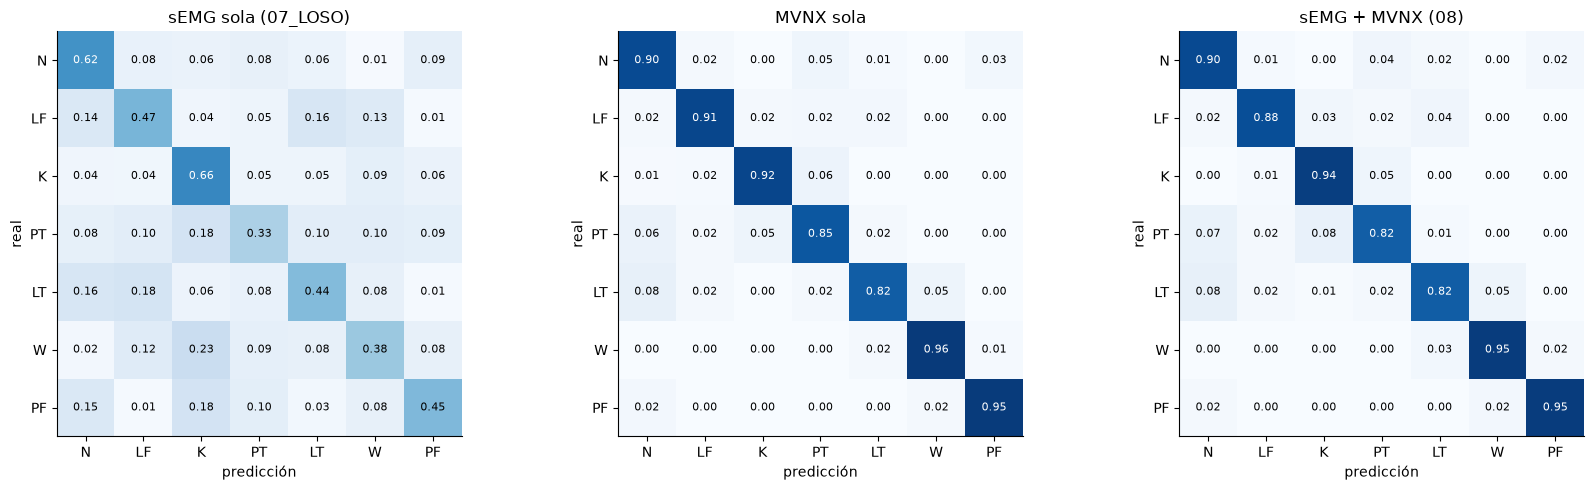
\includegraphics[width=\linewidth]{fig_cm_semg_mvnx.png}
  \caption{Matrices de confusión normalizadas por actividad real (12 sujetos juntos) para la sEMG sola, el movimiento solo y su combinación. Con la sEMG ninguna actividad supera el 66\,\% de aciertos y \act{PT} se queda en 33\,\%; con el movimiento la diagonal va de 82 a 96\,\%.}
  \label{fig:cm_fuente}
\end{figure}

El movimiento lleva prácticamente toda la información útil: distingue la altura de la carga (piso o mesa), que es justo lo que la sEMG no ve. \textbf{Desde este punto el proyecto trabajó sólo con MVNX}, lo que además simplifica la adquisición y elimina la sincronización entre equipos.

\subsection{Modelos candidatos con movimiento (Avance 4)}
Con las 30 variables se compararon familias distintas en las mismas ventanas y rondas (Tabla~\ref{tab:candidatos}). El Random Forest recibe 5 estadísticas por variable y ventana (media, desviación, mínimo, máximo y pendiente; 150 características), así que no ve el orden temporal dentro de la ventana. Las redes reciben la ventana completa.

\begin{table}[H]
  \centering
  \small
  \caption{Modelos candidatos con 30 variables de movimiento (LOSO, 12 sujetos, una semilla). El tiempo de las redes con CPC incluye el preentrenamiento. Fuente: Avance~4 y notebook~10.}
  \label{tab:candidatos}
  \begin{tabular}{lccc}
    \toprule
    Modelo & F1 macro & Peor sujeto & Min por ronda \\
    \midrule
    \textbf{Random Forest} (300 árboles)  & \textbf{0.894} $\pm$ 0.026 & 0.823 & 0.2 \\
    GRU con CPC + LP-FT                   & 0.878 $\pm$ 0.020 & \textbf{0.835} & 5.0 \\
    sLSTM desde cero                      & 0.875 $\pm$ 0.028 & 0.816 & 10.1 \\
    sLSTM con CPC + ajuste fino           & 0.871 $\pm$ 0.031 & 0.815 & 13.7 \\
    mLSTM desde cero                      & 0.862 $\pm$ 0.041 & 0.775 & 12.6 \\
    LSTM desde cero                       & 0.854 $\pm$ 0.032 & 0.787 & 3.9 \\
    CNN 1D desde cero                     & 0.801 & --- & --- \\
    LSTM con CPC + ajuste fino            & 0.747 $\pm$ 0.068 & 0.626 & 2.9 \\
    Referencia: regresión logística sobre las medias & 0.615 $\pm$ 0.043 & 0.551 & --- \\
    \bottomrule
  \end{tabular}
\end{table}

Tres resultados orientaron las decisiones siguientes:
\begin{itemize}
  \item \textbf{La GRU con CPC fue la mejor red:} quedó a 0.016 del Random Forest, con la menor desviación entre personas y el mejor peor sujeto, y es la más rápida de preentrenar. Las diferencias entre GRU, sLSTM y mLSTM ($\le 0.016$) son menores que la variación entre sujetos, así que una celda xLSTM más expresiva no justificaba su costo, de dos a tres veces mayor.
  \item \textbf{La representación aprendida sin etiquetas ya separa las actividades:} con la red CPC-GRU congelada y sólo una sonda lineal, el F1 fue de 0.820, contra 0.631 de la misma red sin preentrenar.
  \item \textbf{Ajustar hiperparámetros no cambió el orden:} con configuraciones elegidas en los sujetos 11--12, el Random Forest pasó a 0.893 y la GRU a 0.879.
\end{itemize}

\subsection{Ensambles sobre CPC (Avance 5)}
El Avance~5 combinó representaciones CPC con clasificadores lineales para que cualquier mejora se debiera a la representación. El \textbf{ensamble homogéneo de cinco CPC-GRU} que sólo difieren en la semilla obtuvo un F1 de $0.873 \pm 0.021$ (peor sujeto 0.827). Superó por 0.060 a la mejor sonda individual en los 12 sujetos, porque una sola sonda dependía mucho de la semilla del preentrenamiento. Los ensambles heterogéneos de GRU, LSTM y sLSTM (concatenación, votación suave, \emph{stacking} y \emph{blending}) y un CPC con las tres redes sobre un encoder compartido quedaron entre 0.813 y 0.846. El \emph{blending} ilustró el riesgo de ajustar con un solo sujeto: tuvo el mejor F1 en validación (0.880) y uno de los peores en prueba (0.813).

\subsection{Reducción de variables y sensores}
\label{sec:reduccion}
Un traje de 17 sensores es poco práctico en una planta. Para encontrar el mínimo, las 30 variables se agruparon \emph{según los sensores de los que dependen} (por ejemplo, la flexión del codo necesita los sensores del brazo y del antebrazo) y se aplicó una eliminación hacia atrás, grupo por grupo. El Random Forest, determinista y rápido, guió la búsqueda (37 subconjuntos), y la CPC-GRU midió cada punto de la ruta. La Tabla~\ref{tab:reduccion} muestra los pasos decisivos.

\begin{table}[H]
  \centering
  \small
  \caption{Ruta de reducción de variables (LOSO, 12 sujetos). Los valores de $p$ comparan la CPC-GRU con su versión de 30 variables. Fuente: notebooks~11 y~12.}
  \label{tab:reduccion}
  \begin{tabular}{lccccc}
    \toprule
    Variables que quedan & Var. & Sensores & F1 RF & F1 CPC-GRU & $p$ \\
    \midrule
    Todas                                          & 30 & 17 & 0.894 & 0.878 & --- \\
    Sin posiciones, hombros, pies ni cabeza & 15 & 12 & 0.896 & 0.883 & 0.04 \\
    \textbf{Codos, manos y piernas (EML)}          & \textbf{10} & \textbf{11} & \textbf{0.892} & \textbf{0.873} & 0.79 \\
    Codos y piernas                                & 6  & 9  & 0.860 & 0.861 & 0.05 \\
    Sólo codos                                     & 2  & 4  & 0.714 & 0.740 & $< 0.001$ \\
    \midrule
    EML medidas sólo con los 11 sensores & 10 & 11 & 0.883 & 0.870 & 0.68$^{\dagger}$ \\
    \bottomrule
  \end{tabular}

  \smallskip
  {\footnotesize $^{\dagger}$ Contra EML calculadas por Xsens con los 17 sensores. La única $p < 0.05$ a favor (15 variables) no resiste la corrección por 8 comparaciones.}
\end{table}

El subconjunto \textbf{EML} (flexión de codos, muñecas, caderas y rodillas de ambos lados, más la rapidez de cada mano) conserva el desempeño de las 30 variables con 11 sensores: pelvis y, de cada lado, brazo, antebrazo, mano, muslo y pierna. Los codos son lo único insustituible: quitarlos baja el F1 a $\approx 0.81$ en cualquier paso. Como las variables de Xsens usan el modelo de cuerpo completo, se recalcularon también \emph{sólo} con las orientaciones de los 11 sensores. Los ángulos coincidieron con los de Xsens (correlación $\ge 0.997$; error mediano $\le 0.4^\circ$) y la CPC-GRU no perdió desempeño (0.870).

\subsection{Modelo final}
\label{sec:final}
Se eligió como modelo final la \textbf{CPC-GRU con las 10 variables EML}, con la configuración de la Sección~\ref{sec:cpc}: encoder causal, GRU de 2 capas (256), cabeza lineal sobre $c_T$ y LP-FT (725\,415 parámetros). Los criterios fueron, en orden: (1) F1 macro en personas nuevas; (2) estabilidad entre personas; (3) desempeño con pocas etiquetas, porque anotar es la parte más cara de llevar el sistema a una planta; y (4) costo y viabilidad en tiempo real (modelo causal, pocos sensores). El ensamble de semillas del Avance~5 alcanza el mismo F1 con 30 variables y 17 sensores, pero cuesta cinco preentrenamientos; el modelo final logra ese desempeño con un solo preentrenamiento y 6 sensores menos.

% =====================================================================
\section{Resultados y validación}
% =====================================================================

\subsection{Desempeño con todas las etiquetas frente a las referencias}
El Avance~3 fijó los umbrales con los que se juzga un modelo, siempre medidos con el mismo protocolo: un \emph{piso} (el azar, 0.143), un \emph{mínimo aceptable} (el mejor baseline) y la \emph{referencia supervisada} con la misma entrada. La Tabla~\ref{tab:final} ubica el modelo final frente a ellos.

\begin{table}[H]
  \centering
  \small
  \caption{Modelo final frente a los umbrales del proyecto (LOSO, sujetos 1--12, todas las etiquetas).}
  \label{tab:final}
  \begin{tabular}{p{9.6cm}cc}
    \toprule
    Referencia & F1 macro & Peor sujeto \\
    \midrule
    Piso: azar estratificado                                  & 0.143 & --- \\
    Baseline inicial: Random Forest sobre sEMG                & 0.485 & --- \\
    Referencia lineal: regresión logística sobre medias (30 var.) & 0.615 & 0.551 \\
    Referencia supervisada: Random Forest (EML, 10 var.)      & 0.892 $\pm$ 0.029 & 0.804 \\
    \textbf{Modelo final: CPC-GRU + LP-FT (EML, 10 var.)}     & \textbf{0.873} $\pm$ 0.036 & 0.775 \\
    \midrule
    \emph{Artículo de referencia:} BiLSTM, 13 sujetos $\to$ 1 sujeto nuevo \parencite{bassani2025} & 0.903 & --- \\
    \bottomrule
  \end{tabular}
\end{table}

El modelo final multiplica por 1.8 el F1 del baseline con sEMG y supera ampliamente a la referencia lineal. Frente al Random Forest con la misma entrada queda a 0.019, una diferencia consistente: el Random Forest gana en 11 de 12 sujetos ($p = 0.005$). La Figura~\ref{fig:sujetos} muestra que la mayor variación está \emph{entre personas}: el F1 de la CPC-GRU va de 0.775 (sujeto~2) a 0.908 (sujeto~4), y ambos modelos coinciden en cuál es el sujeto más difícil. \textbf{Con todas las etiquetas, por lo tanto, CPC no supera al modelo supervisado}; el resultado coincide con lo reportado por \textcite{haresamudram2021}.

\begin{figure}[H]
  \centering
  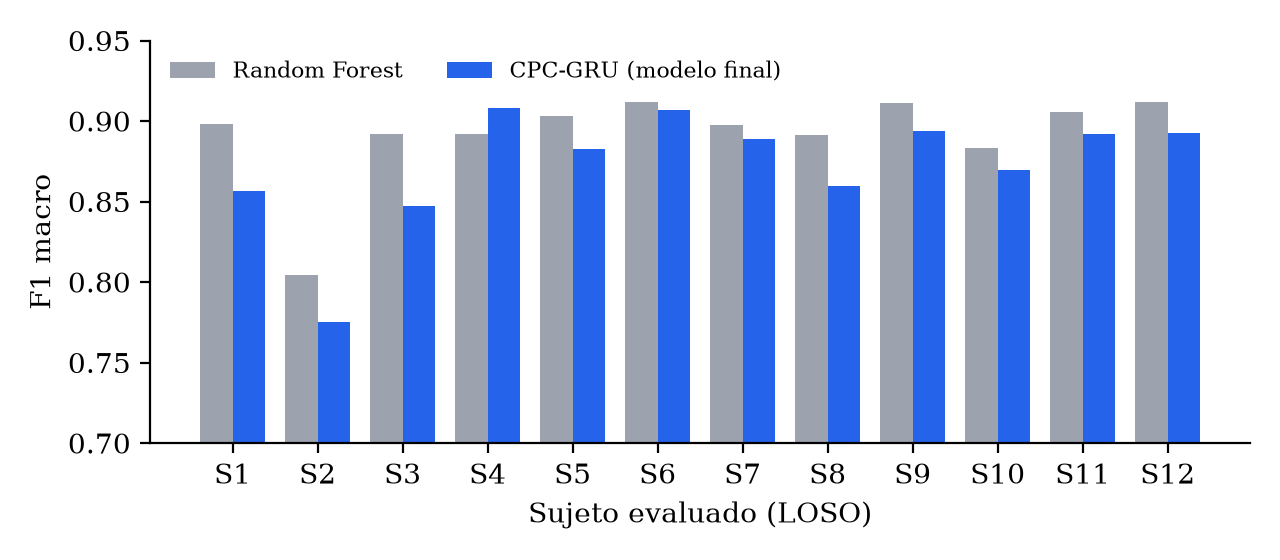
\includegraphics[width=0.86\linewidth]{fig_f1_sujeto.png}
  \caption{F1 macro de cada sujeto evaluado en LOSO, con las 10 variables EML y todas las etiquetas. Cada par de barras es una persona que ningún modelo vio durante el entrenamiento.}
  \label{fig:sujetos}
\end{figure}

\subsection{Errores por actividad y su significado}
La Tabla~\ref{tab:clase} y la Figura~\ref{fig:cm_final} desglosan el desempeño del modelo final por actividad, con las predicciones de los 12 sujetos juntas (F1 macro agrupado de 0.876).

\begin{table}[H]
  \centering
  \small
  \caption{F1 por actividad del modelo final (predicciones de los 12 sujetos evaluados).}
  \label{tab:clase}
  \begin{tabular}{lccccccc}
    \toprule
    & \act{N} & \act{LF} & \act{K} & \act{PT} & \act{LT} & \act{W} & \act{PF} \\
    \midrule
    F1 & 0.917 & 0.837 & 0.914 & 0.821 & 0.823 & 0.933 & 0.889 \\
    \bottomrule
  \end{tabular}
\end{table}

\begin{figure}[H]
  \centering
  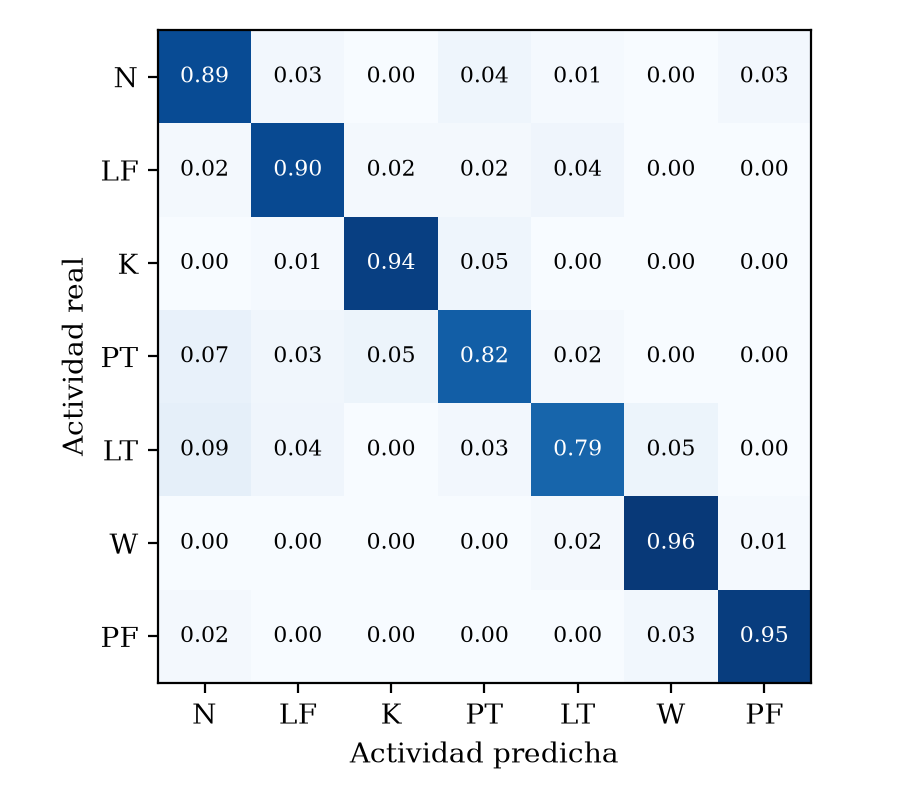
\includegraphics[width=0.52\linewidth]{fig_cm_final.png}
  \caption{Matriz de confusión del modelo final, normalizada por actividad real (cada fila suma 1; 40\,944 ventanas de los 12 sujetos evaluados).}
  \label{fig:cm_final}
\end{figure}

Los aciertos van de 79\,\% (\act{LT}) a 96\,\% (\act{W}). Los errores se concentran en pocos pares:
\begin{itemize}
  \item \textbf{\act{LT} $\to$ \act{N} (8.7\,\%) y \act{PT} $\to$ \act{N} (7.1\,\%):} levantar y colocar en la mesa empiezan y terminan en la postura neutral, y son las actividades más breves (mediana de 1.6 y 2.2~s).
  \item \textbf{\act{PT} $\to$ \act{K} (5.3\,\%) y \act{K} $\to$ \act{PT} (4.6\,\%):} las dos sostienen la carga frente al cuerpo a media altura.
  \item \textbf{\act{LT} $\to$ \act{W} (5.2\,\%):} después de tomar la carga de la mesa suele caminarse con ella.
\end{itemize}

Para un análisis ergonómico, el error más costoso sería confundir una actividad a nivel de piso con una a nivel de mesa, porque se subestimaría la flexión del tronco. Esa confusión es casi nula (\act{PF} $\leftrightarrow$ \act{LT} $\le 0.1$\,\%), y tampoco se confunde caminar con estar quieto (\act{W} $\to$ \act{N}: 0\,\%). Los errores son, sobre todo, \textbf{de frontera entre actividades consecutivas}: el modelo acierta qué ocurre, pero puede adelantar o retrasar el cambio una fracción de segundo. En una aplicación que acumula exposición a lo largo de una jornada, ese tipo de error afecta menos que una confusión entre niveles.

\paragraph{¿Dónde está el techo?} Dos diagnósticos descartaron que el límite estuviera en la lectura de la representación. Una cabeza MLP con 15 veces más parámetros no mejoró (0.876, $p = 0.62$), y el F1 en entrenamiento también se quedó en $\approx 0.90$. Resumir toda la ventana con atención en lugar de usar $c_T$ empató (0.874, $p = 0.97$), y la atención aprendió a concentrar el 61\,\% de su peso en el último segundo. La causa probable está en los datos: el \textbf{89.6\,\% de las ventanas de 4~s cruza una transición} entre actividades, porque las acciones duran entre 1.6 y 4.4~s.

\subsection{Validación en el escenario de pocas etiquetas}
\label{sec:pocas}
El objetivo central del proyecto era medir si el preentrenamiento sin etiquetas compensa tener pocas anotaciones. El experimento (notebook~17) usó el mismo LOSO con un diseño fijado antes de ver los resultados:

\begin{itemize}
  \item CPC se preentrena en cada ronda sólo con las ventanas sin etiqueta de los 10 sujetos de entrenamiento, y su parada temprana usa la pérdida InfoNCE, no etiquetas.
  \item Se toman al azar 1, 2, 5, 10, 25, 50 o 100 ventanas etiquetadas por actividad, con 10 repeticiones por tamaño; todos los modelos reciben exactamente las mismas ventanas.
  \item Los hiperparámetros se eligen con validación cruzada dentro de esas mismas etiquetas, y se evalúa con todas las ventanas del sujeto no visto.
  \item \textbf{Criterio de superioridad:} F1 medio mayor, $p < 0.05$ en Wilcoxon con corrección de Holm sobre 21 comparaciones, y mejora en al menos 9 de 12 sujetos.
  \item \textbf{Controles:} la misma red entrenada desde cero y un encoder aleatorio congelado con las mismas cabezas.
\end{itemize}

\begin{table}[H]
  \centering
  \small
  \caption{F1 macro (media de 12 sujetos y 10 repeticiones) según el número de ventanas etiquetadas por actividad, con las 10 variables EML. Fuente: notebook~17; la columna ``todas'' proviene del notebook~11.}
  \label{tab:pocas}
  \setlength{\tabcolsep}{4.5pt}
  \begin{tabular}{lcccccccc}
    \toprule
    Ventanas por actividad & 1 & 2 & 5 & 10 & 25 & 50 & 100 & todas \\
    \midrule
    CPC-GRU + LP-FT   & 0.368 & 0.473 & \textbf{0.620} & \textbf{0.707} & 0.769 & 0.800 & 0.827 & 0.873 \\
    Random Forest     & 0.323 & 0.407 & 0.513 & 0.611 & 0.722 & 0.777 & 0.816 & 0.892 \\
    Diferencia        & $+0.045$ & $+0.066$ & $\mathbf{+0.107}$ & $\mathbf{+0.096}$ & $+0.047$ & $+0.023$ & $+0.011$ & $-0.019$ \\
    ¿Significativa (Holm)? & sí & sí & sí & sí & no & no & no & --- \\
    \bottomrule
  \end{tabular}
\end{table}

\begin{figure}[H]
  \centering
  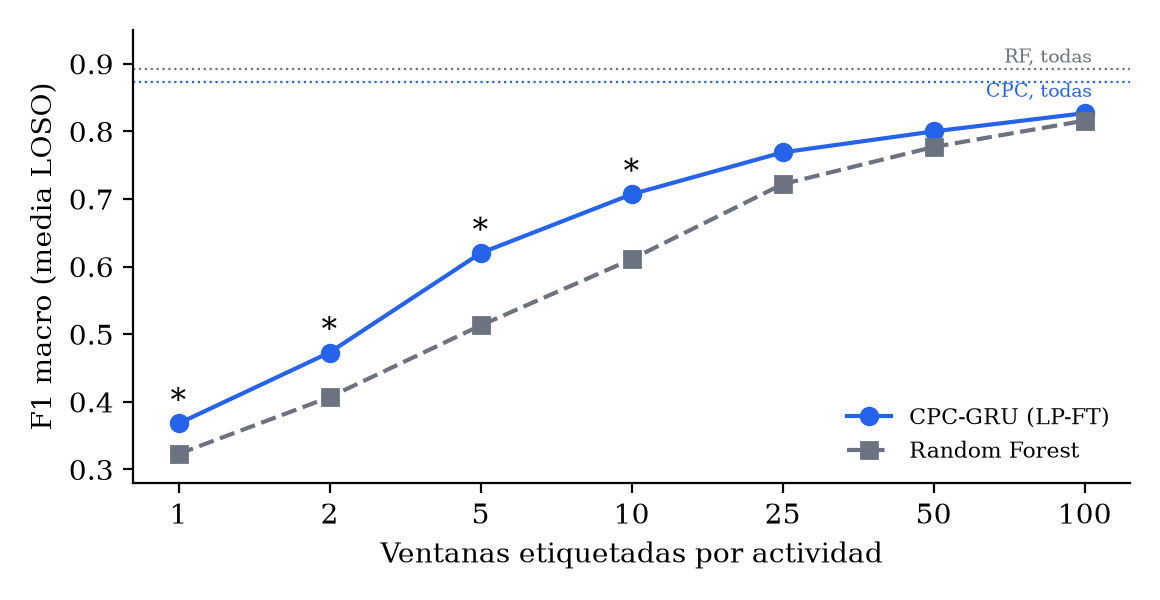
\includegraphics[width=0.78\linewidth]{fig_pocas_etiquetas.png}
  \caption{Curva de etiquetas: F1 macro en un sujeto nuevo según las ventanas etiquetadas por actividad (eje categórico). Las líneas punteadas marcan el desempeño con todas las etiquetas. Los asteriscos señalan las diferencias significativas tras la corrección de Holm.}
  \label{fig:pocas}
\end{figure}

La Tabla~\ref{tab:pocas} y la Figura~\ref{fig:pocas} muestran el resultado principal del proyecto. \textbf{Con 10 ventanas etiquetadas por actividad o menos} (entre 7 y 70 ventanas en total, menos del 0.2\,\% de las etiquetas de entrenamiento), la CPC-GRU supera al Random Forest por 0.045 a 0.107 de F1, en 11 o 12 de los 12 sujetos. Para igualar lo que CPC logra con 5 y 10 ventanas por actividad, el Random Forest necesita unas 11 y 22: \textbf{alrededor de 2.2 veces más etiquetas}. Desde 25 ventanas por actividad la ventaja se reduce y deja de ser significativa, y con todas las etiquetas el orden se invierte.

\paragraph{La ventaja se debe al preentrenamiento.} La misma red entrenada desde cero queda sobre la curva del Random Forest (0.615 contra 0.611 con 10 ventanas), y la CPC-GRU la supera de forma significativa hasta con 25 ventanas por actividad. Con un encoder aleatorio congelado, CPC gana por 0.07 a 0.16 desde 2 ventanas por actividad, en los 12 sujetos. La arquitectura sola no da ventaja; la da lo que CPC aprende sin etiquetas.

\paragraph{Basta congelar la red.} Congelar CPC y entrenar sólo una cabeza lineal, entrenar sólo el MLP de \textcite{haresamudram2021} o ajustar la red completa (LP-FT) difieren en $\le 0.016$ en todos los tamaños. Con 2 ventanas por actividad, la validación eligió cero épocas de ajuste fino en el 76\,\% de los casos.

\paragraph{Dónde gana.} Con 10 ventanas por actividad, la ventaja se concentra en \act{K} ($+0.26$), \act{PT} ($+0.22$) y \act{LT} ($+0.13$), actividades que se distinguen por cómo evoluciona el movimiento más que por la postura promedio. En \act{W} y \act{LF} hay empate, y en \act{PF} gana el Random Forest ($-0.04$). La ventaja es consistente, pero no universal: en el sujeto~8 el Random Forest gana desde 5 ventanas por actividad.

\subsection{Validaciones complementarias}
\begin{itemize}
  \item \textbf{Número de sujetos.} Con las 10 variables de \textcite{bassani2025} (8 de movimiento y 2 de sEMG), la CPC-GRU obtuvo 0.880, igual que con las 30 variables de movimiento ($p = 0.57$). Entrenarla con 4, 6, 8 y 10 personas dio 0.826, 0.852, 0.868 y 0.880: la curva todavía no se aplana, y más sujetos probablemente ayudarían.
  \item \textbf{Comparación con el artículo de referencia.} \textcite{bassani2025} reportan un F1 de 95.7\,\% con una partición aleatoria 70--30 de las ventanas. Con nuestros datos, esa partición sólo sube el F1 en $\approx 0.03$ (CPC-GRU 0.900; Random Forest 0.919), aunque el 90.9\,\% de las ventanas de prueba tiene en entrenamiento una vecina que comparte el 87.5\,\% de sus instantes. Por esa fuga, la cifra comparable con nuestro LOSO es la de su sujeto nuevo (0.903), que está dentro del rango de nuestros sujetos.
\end{itemize}

% =====================================================================
\section{Implementación y operación}
% =====================================================================
El proyecto no se ha desplegado. Esta sección separa lo que ya existe (reproducibilidad) de una \textbf{propuesta} de despliegue que se desprende de los resultados y que no se ha validado.

\subsection{Reproducibilidad del trabajo}
\begin{itemize}
  \item \textbf{Entorno:} el repositorio \texttt{human-activity-recognition} usa \texttt{uv} con Python~3.13 y PyTorch \parencite{paszke2019}; los modelos clásicos usan scikit-learn \parencite{pedregosa2011}. Hay perfiles para CPU o Apple Silicon (MPS) y para GPU NVIDIA.
  \item \textbf{Datos:} no se versionan. El README indica qué archivo de Zenodo descargar y dónde descomprimirlo, con una estructura de carpetas verificable.
  \item \textbf{Ejecución reanudable:} cada ronda LOSO guarda sus pesos (\texttt{.pt}) y sus predicciones y tiempos (\texttt{.json}). Una corrida interrumpida continúa donde se quedó, y los modelos entrenados se conservan para reutilizarse.
  \item \textbf{Controles automáticos:} los notebooks se detienen si las ventanas evaluadas difieren de las de experimentos previos, si un modelo recargado no reproduce sus predicciones (se exigió el 100\,\% de acuerdo) o si cambiar la señal después de $T/2$ altera la salida antes de $T/2$, lo que comprobaría que el modelo no es causal.
  \item \textbf{Trazabilidad:} cada experimento vive en un notebook numerado con su pregunta, su diseño, sus resultados y sus conclusiones, integrado al repositorio mediante solicitudes de cambio (\emph{pull requests}).
\end{itemize}

\subsection{Propuesta de arquitectura de despliegue}
Los resultados sugieren un sistema como el de la Figura~\ref{fig:despliegue}:

\begin{enumerate}
  \item \textbf{Adquisición:} 11 sensores inerciales (pelvis y, de cada lado, brazo, antebrazo, mano, muslo y pierna) con fusión de orientación de calidad comparable a la de Xsens.
  \item \textbf{Preprocesamiento en el borde:} calibración sensor--segmento en una postura neutral al inicio de la sesión; cálculo de las 8 flexiones articulares y de la aceleración de cada mano; pasa-bajas de 4.8~Hz y remuestreo a 12~Hz.
  \item \textbf{Inferencia:} un búfer circular de 48 pasos (4~s) y una clasificación cada 0.5~s con la CPC-GRU. Como el modelo es causal y tiene $\approx 0.7$~millones de parámetros, puede correr en un equipo portátil o en un servidor local; su latencia todavía no se ha medido.
  \item \textbf{Salida:} una secuencia de actividades con marca de tiempo, que alimenta un análisis ergonómico (frecuencia de levantamientos desde el piso, tiempo con carga sostenida, etc.).
\end{enumerate}

\begin{figure}[H]
\centering
\begin{tikzpicture}[
  font=\footnotesize,
  box/.style={draw, rounded corners=2pt, align=center, minimum height=1.0cm, text width=2.35cm, inner sep=3pt},
  arr/.style={-{Stealth[length=2mm]}, thick}]
  \node[box, fill=gray!10] (s) {11 IMU\\ orientación y aceleración};
  \node[box, fill=blue!8, right=0.4cm of s] (p) {Calibración, 10 variables, 12 Hz};
  \node[box, fill=blue!8, right=0.4cm of p] (m) {Búfer de 4 s\\ CPC-GRU causal\\ (cada 0.5 s)};
  \node[box, fill=orange!15, right=0.4cm of m] (o) {Actividades con marca de tiempo};
  \node[box, fill=green!10, below=0.55cm of m, text width=6.2cm] (mon) {Monitoreo: deriva de entradas, distribución de predicciones, auditoría con pocas etiquetas, readaptación de CPC sin etiquetas};
  \draw[arr] (s) -- (p); \draw[arr] (p) -- (m); \draw[arr] (m) -- (o);
  \draw[arr, dashed] (m) -- (mon); \draw[arr, dashed] (p.south) -- (p.south |- mon.north);
\end{tikzpicture}
\caption{Propuesta de arquitectura de despliegue (no validada). Las flechas punteadas indican el flujo de monitoreo.}
\label{fig:despliegue}
\end{figure}

\subsection{Requisitos para producción}
\begin{itemize}
  \item \textbf{Validación previa:} evaluar el modelo final, entrenado con los 12 sujetos, en los sujetos 13 y 14, y medir su latencia en el equipo de destino.
  \item \textbf{Sensores:} medir cuánto ruido, deriva o desfase de calibración tolera el modelo antes de perder desempeño. El proyecto sólo comprobó que errores de 1 a 4$^\circ$ (percentil 95) no cambian el F1.
  \item \textbf{Adaptación a una planta nueva:} grabar varias horas de trabajo sin etiquetas para readaptar el preentrenamiento CPC y anotar unas 10 a 50 ventanas por actividad para entrenar la cabeza lineal. Es el escenario en el que el proyecto midió la ventaja de CPC.
\end{itemize}

\subsection{Monitoreo}
\begin{itemize}
  \item \textbf{Deriva de entradas:} comparar los cuantiles de cada variable con los del escalador de entrenamiento; una desviación sostenida indica descalibración o un sensor desplazado.
  \item \textbf{Deriva de predicciones:} vigilar la proporción de cada actividad por turno y la tasa de cambios entre actividades, que crece cuando el modelo oscila en las fronteras.
  \item \textbf{Autosupervisión como señal:} la pérdida InfoNCE se puede calcular sin etiquetas en los datos nuevos; si sube, la representación ya no describe bien el movimiento de esa población.
  \item \textbf{Auditoría periódica:} anotar una muestra pequeña (unas 10 ventanas por actividad) para estimar el F1 real y decidir si conviene volver a entrenar la cabeza.
\end{itemize}

% =====================================================================
\section{Conclusiones}
% =====================================================================

\subsection{Hallazgos principales}
\begin{enumerate}
  \item \textbf{La fuente de información importa más que el modelo.} La sEMG de los brazos se queda en un F1 macro de 0.44--0.49 con cualquier modelo; el movimiento llega a $\approx 0.88$, y agregar la sEMG no mejora ($-0.006$, $p = 0.15$).
  \item \textbf{Bastan 11 sensores.} Diez variables (flexión de codos, muñecas, caderas y rodillas, más la rapidez de las manos) conservan el desempeño de las 30, y pueden calcularse sólo con las orientaciones de 11 sensores sin pérdida para la CPC-GRU (0.870).
  \item \textbf{Con todas las etiquetas, CPC queda cerca del modelo supervisado, pero no lo supera.} El modelo final obtiene $0.873 \pm 0.036$ contra $0.892$ del Random Forest con la misma entrada.
  \item \textbf{Con pocas etiquetas, CPC es mejor.} Con 10 ventanas etiquetadas por actividad o menos, supera al Random Forest por hasta 0.107 de F1 en 11 o 12 de 12 sujetos. La ventaja se debe al preentrenamiento y equivale a necesitar alrededor de la mitad de las etiquetas.
  \item \textbf{El techo está en los datos, no en el clasificador.} Ni una cabeza más grande ni resumir toda la ventana mejoran. Los errores restantes son de frontera entre actividades breves y consecutivas, y casi nunca confunden actividades de piso con actividades de mesa.
\end{enumerate}

\subsection{Limitaciones}
\begin{itemize}
  \item \textbf{Sin prueba final:} todos los resultados provienen de LOSO con los sujetos 1--12, y el subconjunto EML se eligió con esos mismos sujetos, por lo que su F1 es algo optimista. Además, un notebook exploratorio temprano llegó a mostrar resultados de los sujetos 13 y 14, así que su evaluación no será completamente ciega.
  \item \textbf{Una sola semilla} en la mayoría de las comparaciones de redes. Diferencias de $\pm 0.01$ pueden ser ruido; la LSTM desde cero llegó a variar de 0.61 a 0.86 en un mismo sujeto según la semilla y la parada temprana.
  \item \textbf{Población pequeña y homogénea:} 14 adultos jóvenes en laboratorio, con dos mujeres. La curva por número de sujetos todavía no se aplana.
  \item \textbf{Escenario de pocas etiquetas idealizado:} ventanas balanceadas por actividad y tomadas de los 10 sujetos; un etiquetado real tendería a concentrarse en pocas personas. Además, el preentrenamiento llegó al tope de 20 épocas en 10 de 12 rondas.
  \item \textbf{Sensores simulados a partir del MVNX:} las orientaciones ya pasaron por la fusión de Xsens, y la calibración se estimó ensayo por ensayo, lo que es más favorable que una calibración real por sesión.
\end{itemize}

\subsection{Trabajo futuro}
\begin{itemize}
  \item Evaluar el modelo final, entrenado con los 12 sujetos, en los sujetos reservados 13 y 14.
  \item Ejecutar el barrido de duración de ventana, horizonte de predicción y dimensiones latentes, con su visualización t-SNE, que ya está preparado (notebook~13), y confirmar las configuraciones finalistas con tres semillas.
  \item Usar ventanas o etiquetas acordes a la duración de las acciones ($\approx 2$~s) para atacar los errores de frontera.
  \item Medir la sensibilidad del sistema de 11 sensores a ruido, deriva y desfase de calibración.
  \item Explorar \emph{Contrastive Active Inference} \parencite{mazzaglia2021} como alternativa autosupervisada a CPC, con el mismo protocolo.
\end{itemize}

% --- Declaración de uso de IA ---
\section*{Declaración de uso de inteligencia artificial}
Se utilizó \textcite{anthropic2026claude} como apoyo para generar y optimizar el código de los notebooks (preparación de datos, protocolo LOSO, modelos CPC y análisis) y para redactar y editar este artículo a partir de los resultados del repositorio. El equipo definió los experimentos, verificó que las cifras coinciden con las de los notebooks y revisó las figuras y su interpretación. La responsabilidad final sobre el contenido entregado recae en los autores.

% --- Referencias ---
\printbibliography[title={Referencias}]

% --- Anexos ---
\clearpage
\appendix

\section{Variables de movimiento}
\label{anx:variables}
\begin{table}[H]
  \centering
  \small
  \caption{Las 30 variables MVNX usadas desde el Avance~4. En negritas, las 10 del subconjunto EML del modelo final.}
  \begin{tabular}{p{3.0cm}p{8.2cm}p{3.0cm}}
    \toprule
    Categoría & Variables & Grupo de sensores \\
    \midrule
    Postura (14) & Flexión del tronco y del cuello; de cada lado: flexión y abducción del hombro, \textbf{flexión de codo}, \textbf{de muñeca}, \textbf{de cadera} y \textbf{de rodilla} & Tronco, cabeza, hombros, \textbf{codos}, \textbf{manos}, \textbf{piernas} \\
    Alturas y alcance (6) & Altura de pelvis, cabeza y cada mano; distancia horizontal de cada mano a la pelvis & Posiciones globales (17 sensores) \\
    Velocidades (6) & Rapidez horizontal y velocidad vertical de la pelvis; \textbf{rapidez de cada mano}; giro de la pelvis; velocidad angular del tronco & Pelvis, \textbf{manos}, tronco \\
    Apoyo (4) & Contacto de talón y punta de cada pie & Pies \\
    \bottomrule
  \end{tabular}
\end{table}

\section{Experimentos que no prosperaron}
\label{anx:descartes}
\begin{table}[H]
  \centering
  \small
  \caption{Experimentos realizados cuyos resultados no se adoptaron (LOSO, sujetos 1--12).}
  \begin{tabular}{p{5.2cm}p{9.3cm}}
    \toprule
    Experimento & Resultado y motivo del descarte \\
    \midrule
    CPC sobre sEMG con GRU, LSTM, sLSTM y mLSTM; horizontes, tipos de negativos y 12 o 25~Hz (notebooks~01--07) & Mejor configuración: sLSTM, horizonte de 1~s y negativos del mismo sujeto, con F1 0.437. La señal limitaba el resultado. \\
    sEMG + movimiento & 0.880 contra 0.885 con movimiento solo; la sEMG no aportó. \\
    LSTM con CPC y ajuste fino original & 0.747; el ajuste fino deformó la representación (motivó LP-FT). \\
    mLSTM y CNN 1D desde cero & 0.862 y 0.801, por debajo de la GRU con CPC. \\
    BiLSTM como red de contexto de CPC & Descartado en teoría: su lectura hacia atrás ya conoce el futuro que CPC debe predecir. No se entrenó. \\
    Ensambles heterogéneos y CPC con tres redes de contexto & 0.813--0.846, por debajo del ensamble de semillas (0.873). \\
    Cabeza MLP en lugar de lineal & 0.876 contra 0.873 ($p = 0.62$), con 15 veces más parámetros. \\
    \emph{Pooling} promedio o con atención sobre $c_1,\dots,c_T$ & Promedio 0.840 ($p = 0.002$, peor); atención 0.874 ($p = 0.97$). \\
    Submuestreo de \act{N} en lugar de pesos por clase & $-0.008$ con ajuste fino lineal ($p = 0.08$). \\
    Ventanas de 1~s sin traslape con 30 variables + sEMG & CPC-GRU 0.861, peor que con 4~s; el Random Forest llegó a 0.908, pero con sEMG y 17 sensores. \\
    \bottomrule
  \end{tabular}
\end{table}

\section{Configuración del modelo final}
\label{anx:config}
\begin{table}[H]
  \centering
  \small
  \caption{Hiperparámetros de la CPC-GRU final.}
  \begin{tabular}{p{4.5cm}p{9.8cm}}
    \toprule
    Elemento & Valor \\
    \midrule
    Entrada & 10 variables EML, 48 pasos (4~s a 12~Hz), etiqueta del instante final \\
    Encoder & 3 Conv1d causales ($10 \to 32 \to 64 \to 128$), núcleo 3, ReLU, \emph{dropout} 0.2 \\
    Red de contexto & GRU de 2 capas, 256 unidades, \emph{dropout} 0.2 \\
    Preentrenamiento CPC & InfoNCE, horizontes de 1 a 12 pasos (1~s), 128 negativos del mismo sujeto, ventanas sin etiqueta cada 2~s; parada temprana con sonda lineal en la validación interna \\
    Cabeza & LayerNorm(256) $\to$ Dropout 0.2 $\to$ Linear(256, 7) sobre $c_T$ \\
    Ajuste supervisado & LP-FT; tasa de aprendizaje $10^{-4}$ (red) y $10^{-3}$ (cabeza); hasta 30 épocas, paciencia 5; entropía cruzada con pesos por clase \\
    Parámetros & 725\,415 \\
    Tiempo por ronda & $\approx$ 4--7 min en Apple Silicon (MPS), incluido el preentrenamiento \\
    \bottomrule
  \end{tabular}
\end{table}

\end{document}
